%*****************************************
\chapter{Peso molecolare medio}\label{ch:PM}
%*****************************************
Per ottenere il peso molecolare di una molecola bisogna vedere la tavola periodica \ref{chp:Tavolaperiodica} a pagina \pageref{chp:Tavolaperiodica}.
Ad esempio:

\begin{figure}
\subfloat[][\emph{Molecola}\label{fig:Mol}]%
{%
\setchemfig{atom sep = 2em}%
\chemfig{\vphantom{C}-[@{op,.75}]CH_2-C(-[2]CH_3)(-[6]CH_3)-[@{cl,.25}]}%
\polymerdelim[indice n]{op}{cl}}\quad
\subfloat[][\emph{Peso molecolare}\label{fig:PMmol}]%
{%
\begin{minipage}[b]{0.4\textwidth}
\begin{equation}
4*\underbrace{12}_{C} + 8*\underbrace{1}_{H} = 56\unit{\g/\mol}
\end{equation}
\end{minipage}%
}
\end{figure}

Dunque in generale si può scrivere la regola:
\begin{equation}
P.M. = P.M. * n
\label{eqn:PM}
\end{equation}

Nella realtà però, non è possibile descrivere il \ac{PM} in quanto non è detto che le catene polimeriche siano ideale e composte sempre allo stesso modo.
Dunque si stima il \ac{PMM}.

In generale la curva che descrive il \ac{PMM} per un materiale polimerico non è descritta come gaussiana ma come una curva del tipo

\begin{figure}
\centering
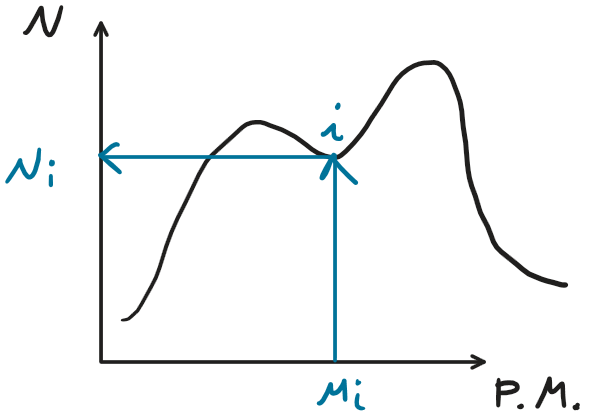
\includegraphics[width = 0.7\textwidth]{gfx/PM}
\caption{Esempio di distribuzione dei pesi molecolari in funzione del numero di moli}
\label{fig:PM}
\end{figure}

$N$ rappresenta il numero di moli con il dato peso molecolare.
In genere si hanno due massimi nella distribuzione del peso molecolare.
Le frazioni a peso molecolare più basso servono a dare al materiale delle proprietà viscose basse.
Quelle a peso molecolare alto per dare le caratteristiche meccaniche.

\section{Peso molecolare medio numerico}
Un primo parametro di caratterizzazione del polimero può essere il peso molecolare medio.
Se 
\begin{equation}
\begin{split}
W &:= \textup{Peso del campione}\\
N &:= \textup{numero totale di moli nel campione}\\
\bar{M}_n &:= \textup{Peso molecolare medio numerico}\\
\phi_i &:= \textup{Frazione molecolare}\\
\bar{M}_n &= \sum_i{\frac{W_i}{N}} = \frac{\sum_i{N_iM_i}}{N} = \sum_i{\frac{N_i}{N}M_i} = \sum_i{\phi_iM_i}
\end{split}
\end{equation}  

\section{Peso molecolare medio ponderale}
\begin{equation}
\begin{split}
\bar{M}_w &:= \textup{peso molecolare medio ponderale}\\
\psi_i &:= \textup{Frazione ponderale}\\
\bar{M}_w &= \sum_i{\frac{W_i}{W}M_i} = \frac{\sum_i{N_iM_i^2}}{W} = \sum_i{\frac{N_iM_i^2}{N_iM_i}} 
\end{split}
\end{equation}

Si può dimostrare che il peso medio ponderale è maggiore del peso medio numerico.
I due pesi medi molecolari sono uguali nel momento in cui entrambi sono uguali a un certo valore $M$.
Si può allora definire un \ac{IPD} detto anche poli-dispersità.
\begin{equation}
IDP = \frac{\bar{M}_w}{\bar{M}_n} \geq 1
\label{eqn:IDP}
\end{equation}
Dalla definizione si osserva che vale $1$ quando il polimero è mono-disperso, poli-disperso altrimenti.

Il peso molecolare medio ponderale è sensibile alle variazioni di frazioni molecolare ad alto peso molecolare.
Il peso molecolare medio numerico sensibile alle variazioni di frazioni molecolari a basso peso molecolare.

\section{Metodi di misura dei pesi molecolari}
Per la misura del peso molecolare di un campione, si scruta la dipendenza della viscosità dal peso molecolare. 
se ne estrae, tramite prove di viscosità, un peso molecolare medio. 
Si può ottenere un'ulteriore misura che permette non solo di valutare i pesi molecolari medi, consentendoci di ottenere direttamente la distribuzione dei pesi molecolari.

Non si possono ricavare con delle misure dirette i pesi molecolari, infatti le misure si realizzano sulla viscosità. 
Si parla di due tipi di viscosità: 
\begin{itemize}
\item viscosità a caldo, dove il materiale viene portato a fusione e ne misura la viscosità
\item viscosità in soluzione, dove si scioglie il materiale in un solvente con viscosità nota e si misura quella del composto misto.
\end{itemize}

\subsection{Melt Flow Index}
Il \ac{MFI} È una misura che viene realizzata attraverso lo stato fluido del materiale di test. Siccome c'è una relazione tra la pressione esercitata e la portata del materiale estruso , si può misurare la viscosità del materiale.

Questo tipo di misura non è ottima in quanto i dati che se ne ottengono sono molto marginali e poco caratteristici. Oltre al fatto che sono molto sporchi per via dello strumento di misurazione.
Nei fluidi polimerici la viscosità, vedi capitolo \ref{chp:MisureViscosità} a pagina \pageref{chp:MisureViscosità}, non può essere rappresentata solo dalla pressione e dalla temperatura. Dimostra che la misura è decisamente limitata nelle sue opportunità.

In generale per un polimero che deve essere stampato ad iniezione la viscosità deve essere abbastanza bassa, dunque il peso molecolare basso e il grado di polemizzazione basso conseguentemente. Ci si aggira attorno a $10\div20\unit{MFI}$.
Bisogna considerare che l'unità di misura per la misurazione \ac{MFI} è espressa come rapporto tra la massa ogni 10 minuti $\left[g/10\,min\right]$.

Questo denota anche la natura della misura ovvero si fa fluire il materiale polimerico all'interno di un capillare, applicando una ben determinata pressione e misurandone la massa caduta su un piatto sotto il capillare. Esistono alcune normative che prevedono delle indicazioni su come viene eseguita questo tipo di prova.

\begin{figure}
\centering
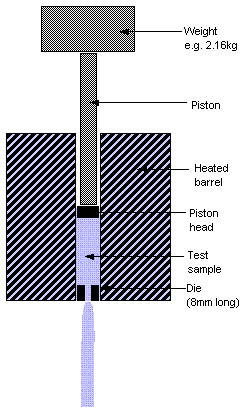
\includegraphics[width = 0.4\textwidth]{gfx/MFI}
\caption{Schematizzazione misura \ac{MFI} \href{https://commons.wikimedia.org/w/index.php?curid=33527584}{by Miladfarhani - Own work, CC BY-SA 3.0}}
\label{fig:MFI}
\end{figure}

Altre tipologie di produzione di materiali plastici chiedono un \ac{MFI} più alto oppure più basso a seconda della tecnologia utilizzata.

Il produttore di materiali plastici sono obbligati a fornire le loro misure \ac{MFI} e qualche temperatura di processo caratteristica del polimero.

Resta evidente come questo tipo di misura non dà alcuna idea sul peso molecolare, se ne dà solo un'indicazione.
Questo indice viene spesso utilizzato come controllo qualità sia in ingresso che in uscita. Si usa anche per controllare se il processo di trasformazione è stato eseguito regolarmente.
Questo perché variazioni di temperatura durante il processo di produzione possono causare dei cambiamenti nello stato dei polimeri comportando così una perdita di qualità nel prodotto. 

\subsubsection{Controllo qualità}
Per il controllo del processo produttivo: sappiamo che il riscaldamento e il raffreddamento del materiale fanno decadere le proprietà meccaniche di quest'ultimo accorciando le catene polimeriche. 
Ciò vuol dire che col decadimento delle catene polimeriche calerà anche il peso molecolare medio , quindi anche la viscosità e per l'appunto le caratteristiche meccaniche. Allora aumenterà \ac{MFI} indicando appunto un erroneo processo di lavorazione.
Stesso concetto che si utilizza quando si vuole aggiungere a della plastica vergine della plastica riciclata. In questo caso allora si parla di \textbf{rimacinaggio} ovvero il processo di recupero dei materiali plastici riciclati.
Ovviamente il materiale che si riutilizza perderà di caratteristiche meccaniche in generale non bisognerebbe superare una percentuale del $20\%$ anche se in pratica si arriva anche al $50\%$.

\section{Peso molecolare medio in viscosità}
\begin{equation}
\bar{M}_v
\end{equation}
Si prende un solvente di tipo organico costituendo una soluzione. Il metodo consiste nella misurazione della viscosità della soluzione.

\begin{figure}
\centering
\subfloat[][\emph{Viscosità della soluzione in funzione della concentrazione}\label{fig:ViscSpec}]
{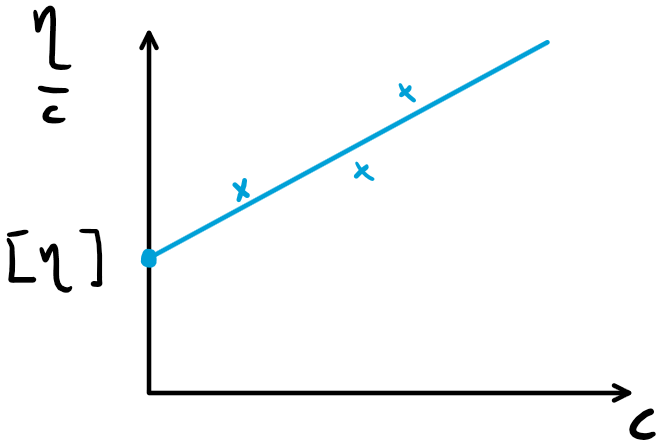
\includegraphics[width = 0.4\textwidth]{gfx/ViscSpec}}\quad
\subfloat[][\emph{Calcolo della viscosità intrinseca}\label{eqn:ViscSpec}]
{%
\begin{minipage}[b]{0.4\textwidth}
\begin{equation}
\begin{split}
\frac{\eta - \eta_0}{\eta_0} &= \eta_{sp}\\
\eta &= \textup{Viscosità della soluzione}\\
\eta_0 &= \textup{Viscosità del solvente}\\
c &= \textup{Concentrazione}
\end{split}
\end{equation}
\end{minipage}%
}
\caption{Calcolo della viscosità specifica del polimero}
\label{def:ViscSpec}
\end{figure}
In letteratura questa viene chiamata sia a viscosità specifica che viscosità intrinseca del polimero.
Da cui si definisce la \textbf{formula di Mark-Houwink}.
\begin{equation}
\left[\eta\right] = KM_v^a
\label{eqn:MarkHounwink}
\end{equation}
Noto il polimero di partenza si possono ricavare $K$ ed $a$ dalla letteratura.
Siccome la viscosità intrinseca si riesce a misurare allora si può ottenere il suo valore $\bar{M}_v$. Tra l'altro risulta che il peso medio in viscosità risulta essere intermedio tra il peso molecolare numerico e il peso molecolare ponderale.

Per la misurazione delle moli si può ottenere una stima tramite dei gruppi terminali se si sanno quali sono i gruppi terminali, mediante analisi chimiche, si possono stimare i numeri delle molecole partendo proprio dalla conta dei terminali.
Per la misura del peso molecolare medio ponderale. Non esiste una misura precisa. Si possono fare delle prove di diffusività della luce: perché le molecole a più alto peso impediscono il passaggio della luce.

\subsection{La GPC}
La \ac{GPC} È una misura di tipo viscoso e non legato a pressione e temperatura come la precedente \ac{MFI}.
Nella pratica si scioglie il polimero in un solvente, dopodiché la soluzione viene pompata in delle colonne di separazione. Nelle colonne di separazioni sono è presente nel gel con alcune sfere porose. Le sfere porose separeranno le molecole ad alto peso molecolare da quelle a basso peso molecolare.
Dunque, le molecole a più alto peso molecolare percorreranno le colonne in minor tempo. Questo perché non entrano all'interno della porosità delle sfere contenute nel gel. Mentre le molecole a più basso peso molecolare vengono "intrappolate" all'interno delle sfere per cui impiegano molto più tempo a percorrere il gel.
La misura Lega il tempo percorso della soluzione. Prima verranno le molecole ad alto peso molecolare e poi le molecole via via più piccole, andando così a descrivere una vera e propria distribuzione di pesi molecolari. 


%************************************************
\chapter{Cristallizzazione}\label{chp:Cristallizzazione}
%************************************************
I cristalli sono materiali solidi i cui elementi costituenti hanno una posizione ben definita.

I materiali polimerici hanno sempre una parte amorfa:
\begin{itemize}
\item Se il materiale cristallizza: una parte di materiale resta amorfa e una parte cristallizza.
\item Se il materiale non cristallizza, tutto il materiale si presenta in forma amorfa. 
\end{itemize}
La cristallinità è il rapporto tra il materiale che ha cristallizzato rispetto alla totalità del materiale.

\begin{equation}
\alpha = \frac{M_c}{M}
\label{eqn:Cristallinità}
\end{equation}
I materiali molto cristallini hanno in genere $\alpha \approx 50 \div 60 \%$.
Fa eccezione il poliossimetilene che è praticamente tutto cristallino $\approx 90\%$ da cui derivano le sue proprietà meccaniche molto importanti. Addirittura troppo importanti, nel senso che spesso il poliossimetilene viene addizionato per evitare la sua totale cristallizzazione in modo tale che sia più tenace agli sforzi.

La restante parte dei materiali, coloro che cristallizzano solo parzialmente, vengono chiamati in gergo \textbf{semi-cristallini}.

\begin{figure}
\centering
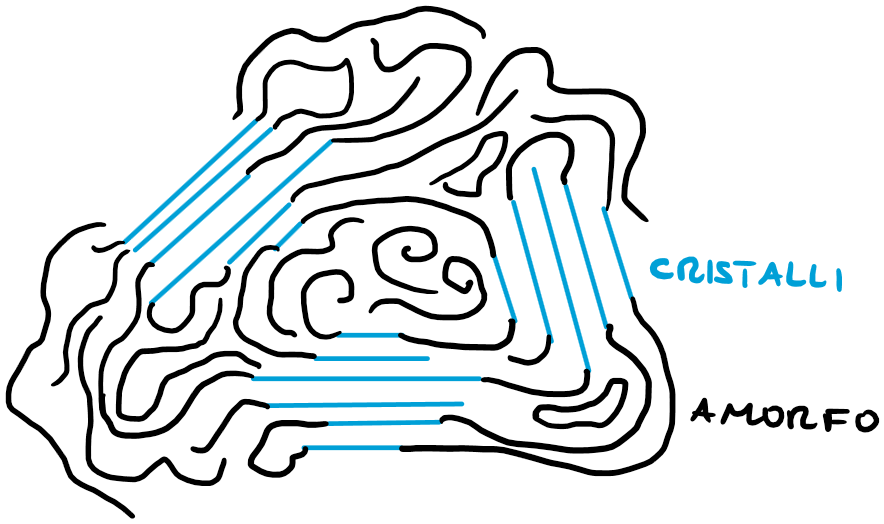
\includegraphics[width = \textwidth]{gfx/Cristallinita}
\caption{Esempio di materiale semi-cristallino}
\label{fig:Cristallinita}
\end{figure}

I cristalli donano particolari caratteristiche meccaniche perché la molecola resta dritta quindi direzionabile rispetto allo sforzo.
Inoltre, la stessa molecola può formare sia più parti cristalline che parti amorfe. Addirittura una stessa catena polimerica può far parte più volte dello stesso cristallo e collegare le parti cristalline tramite zone amorfe.

Uno stesso materiale polimerico può o non può cristallizzare. Ad esempio il \ac{LDPE} è un polietilene poco cristallino. Mentre il \ac{HDPE} è un polietilene ad alta densità da cui ne derivano caratteristiche meccaniche molto interessanti.

I materiali cristallini tendono ad avere una densità più alta per via del maggiore impaccamento delle molecole. Da ciò derivano anche le caratteristiche meccaniche più sviluppate. 

La maggiore resistenza dei materiali cristallini è data dal fatto che se si applica uno sforzo nel senso del cristallo, allora si va ad agire direttamente sui legami principali,di più alta qualità. Evidentemente ci sono dei problemi di anisotropia nel materiale.
Idealmente, si potrebbero migliorare le performance dei cristalli se tra di loro fossero tutti allineati in un'unica direzione. Allora, nonostante il problema di anisotropia, si può pensare di applicare al materiale uno sforzo parallelo alla direzione dei cristalli e quindi riscontrare una resistenza più alta.
La realtà ci dice tutt'altro, infatti essendo che i materiali polimerici non possono cristallizzare totalmente, una quota parte di materiale resta amorfo. Dunque: sebbene esistano i cristalli, gli sforzi esterni tendono ad essere condivisi tra la parte cristallina e la parte amorfa. In questo modo si limitano le caratteristiche meccaniche del materiale.
Nello specifico un materiale particolarmente disorganizzato: ovvero a basso contenuto cristallino; avrà proprietà meccaniche più basse. Invece un materiale più alto grado cristallino risulterà più duro.

Le parti amorfe non sono da eliminare infatti la presenza permette al materiale di risultare più tenace che non un materiale duro ma fragile in questo modo può sopportare determinati tipi di stress in maniera più agevole.
Ciò vale solamente nel caso in cui le parti amorfe hanno un'interfaccia con le parti cristalline.

I cristalli nello specifico presentano delle catene polimeriche particolarmente dritte ed organizzate questo è dovuto all'alta stabilità termodinamica. Dunque è più difficile che le molecole ruotino tra di loro. Siccome tra l'altro c'è una convenienza dal punto di vista energetico allora la zona cristallina risulta più rigida bloccando in maniera diritta le molecole.

Resta il fatto che essendo il materiale termoplastico se scaldato sufficientemente le reticolazioni possono essere sciolte 

\section{Requisiti per la cristallizzazione}
Com'era già stato anticipato, capitolo \ref{chp:Classificazione} a pagina \pageref{chp:Classificazione}: il requisito fondamentale è dato dalla regolarità della macromolecola che deve essere sintetizzata senza errori.
Si ricorda che però questa condizione è necessaria ma non sufficiente.

Prendendo il caso del \ac{PE}, con un grado di polimerizzazione che in genere si attesta attorno a $n \approx 1000 \div 10000$.
Le possibili tipologie di errore sono:
\begin{description}
\item[Impurezze] Se nel relatore oltre all'etilene si presenta qualsiasi altro alcheno a basso peso molecolare si formano degli errori in catena principale.
\item[Ramificazioni] Il \ac{LDPE} presenta parecchie ramificazioni in catena principale mentre il \ac{HDPE} si riesce a sintetizzare particolarmente lineare. Infatti quest'ultimo ne presenta in numero molto limitato e riesce a cristallizzare.Il \ac{HDPE} viene sintetizzato con dei catalizzatori che permettono di abbassare la temperatura di reazione rendendo la reazione più controllabile.
\item[Concatenamenti] Affinché un polimero sia regolare ci deve essere un concatenamento testa-coda regolare. Può succedere che durante la sintesi si abbiano degli errori di sequenza testa-coda.
\item[Stereo-isometria] errore comune peri vinili.  
Questo tipo di errore prevede che nella catena polimerica l'ordine dei sostituenti laterali sia irregolare nel ordine, dovuto principalmente all'ibridazione del carbonio. Allora si parla di polimero \textbf{isotattico} quando la catena è perfettamente regolare. Se alterna il legame frontale con quello posteriore allora si parla di polimero \textbf{sindiotattico}, altrimenti si dice \textbf{atattico} nel caso sia irregolare.
È palese che per la regola della regolarità solo i primi due possono reticolare mentre l'ultimo no.
\end{description}

\begin{figure}
\centering
\setchemfig{atom sep = 2em}
\schemestart
\chemname{\chemfig{\vphantom{C}-[@{op,.75}]**6(---(-C(-[2]CH_3)(-[6]CH_3)-**6(---(-O-C(=[2]O)-O-[@{cl,.25}])---))---)}}{Policarbonato}
\polymerdelim[indice = n]{op}{cl}
\schemestop
\caption{Monomero del policarbonato}
\label{fig:Policarbonato}
\end{figure}

Esistono comunque dei materiali che nonostante siano regolari non cristallizzino. Ad esempio il \ac{PC} (figura \ref{fig:Policarbonato}) è un materiale regolare ma presenta problemi di tipo \textbf{cinetico}. Perché durante il raffreddamento il materiale non ha il tempo per: potersi spostare e raddrizzarsi per poter formare i cristalli a causa alla catena troppo rigida. 
Anche il \ac{PET} presenta un problema analogo. Infatti durante la solidificazione la catena principale non ha tempo di organizzarsi in cristalli. Ciò viene sfruttato a vantaggio per realizzare le bottiglie di plastica. Infatti viene forzato a cristallizzare durante il soffiaggio per ottenere la bottiglia di plastica.
Il fenomeno è dato dal fatto che durante il soffiaggio il materiale viene scaldato e poi stirato. Per cui le molecole hanno tutta l'energia necessaria per adattarsi alla forma data dallo stampo.
Questa viene detta \textbf{cristallizzazione sotto stiro}. 

Un'ulteriore struttura cristallina si chiama \textbf{sferulite} ed è costituita da strati di lamelle cristalline e lamelle di strati amorfi.
Il materiale che presenta tale cristallinità presenta anche un'alta fragilità che può essere uno svantaggio considerando il campo di applicazione di tali materiali.
Un materiale molto cristallino tende a perdere di trasparenza, diventano opalescenti. Perché la luce non filtra attraverso la parte cristallina ma solo attraverso la parte amorfa dunque si ha una ben definita trasparenza in base al materiale.

\begin{quote}
\emph{Si può controllare la cristallinità?}
\end{quote}
Si può controllare la cristallinità, o il grado di cristallinità, tramite il controllo del raffreddamento del materiale una volta prodotto.
Infatti, per anche per un materiale che cristallizza, se il raffreddamento è troppo rapido le molecole non hanno il tempo di organizzarsi in cristallo dunque rimane amorfo.

Dopo il raffreddamento possono sussistere due problematiche:
\begin{enumerate}
\item Siccome la temperatura ambiente è sufficiente a permettere la mobilità delle molecole allora queste tenderanno ad avvicinarsi e ad impaccarsi formando i cristalli. Dunque si ha una deformazione del materiale per cui si perde qualità in tolleranza 
\item Per lo stesso motivo: tentando di bloccare la deformazione del materiale si hanno comunque delle tensioni residue interne a questo.
\end{enumerate}

Altro metodo per evitare una cristallizzazione eccessiva è sfruttare la \textbf{copolimerizzazione} un processo per evitare che il polimero sia troppo regolare e quindi cristallizzi eccessivamente.
\begin{itemize}
\item Ad esempio si può copolimerizzare il \ac{PP} con il \ac{PE} si forma una plastica che ha delle proprietà meccaniche calanti rispetto ai due puri, ma non è completamente cristallino per cui è abbastanza trasparente.
\item Il poliossimetilene viene limitato nella sua cristallinità proprio grazie alla copolimerizzazione, viene polimerizzato con l'ossido di etilene. 
\end{itemize}

\section{Misure di cristallinità}
Ora si vedranno quali sono le misure che permettono di valutare il grado di cristallinità di un materiale polimerico.

Le prime tre che vedremo permettono di conoscere la conformazione di quale tipo di polimero sia ciò dovuto al fatto che la temperatura di fusione è ben caratteristica del singolo polimero.

In generale per conoscere la tipologia di polimero che si sta utilizzando si utilizzano delle analisi termiche.

\subsection{Dilatometria}
Determinare la temperatura di transizione vetrosa è molto complicato tramite la misura della dilatazione della plastica, perché la variazione di comportamento è poco significativa e poco percettibile.

Per realizzare una dillatometria di un materiale cristallino è necessario conoscere a prescindere: il suo comportamento come se fosse completamente cristallino e il suo comportamento come se fosse completamente amorfo.
Allora la dialettometria si realizza tramite lo spostamento della curva del materiale completamente cristallino verso la temperatura ambientale mentre si collega in maniera continua al comportamento del materiale completamente amorfo.

Allora si può definire la cristallinità come:
\begin{equation}
\alpha = \frac{v_a - v_{sc}}{v_a - v_c}
\label{eqn:Dilatometria}
\end{equation}

\begin{figure}
\centering
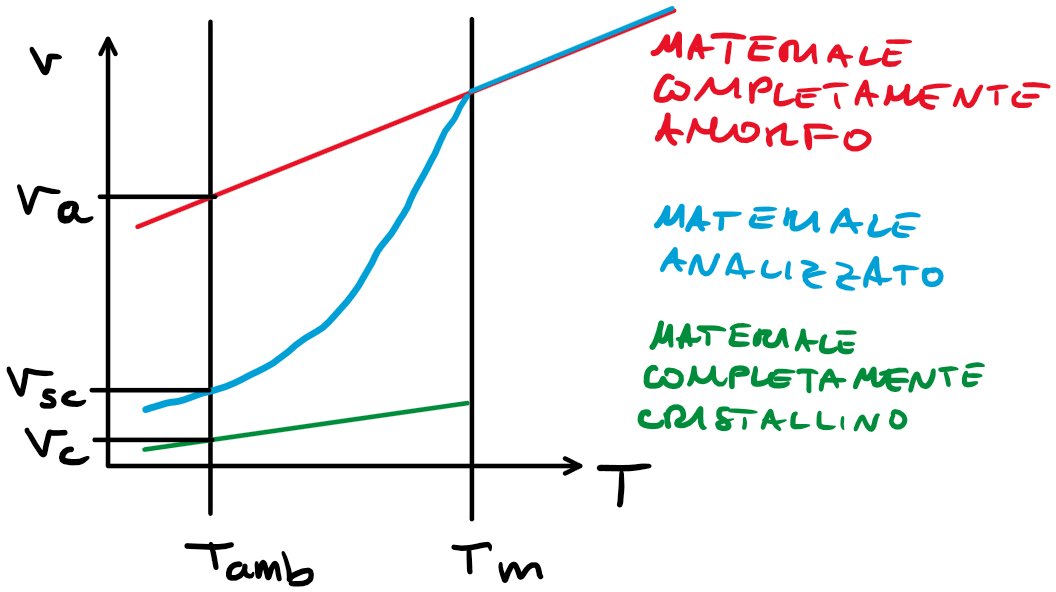
\includegraphics[width = \textwidth]{gfx/Dilatometria}
\caption{Esempio di dilatometria}
\label{fig:Dilatometria}
\end{figure}

\subsection{DSC}
La \ac{DSC} è una prova che si basa su due contenitori con applicati dei riscaldatori: su uno viene messo il materiale di prova; sull'altro si ha il riferimento, che in genere è un gas inerte o che almeno non interagisca col polimero. Si impone una velocità di riscaldamento nota $10\unit{\celsius/\min} \div 20\unit{\celsius/\min}$ se ne misura la potenza termica a cui si sottopone il test.
A questo punto si fa la differenza tra i due riscaldatori. Dunque si ottiene la differenza di potenza termica assorbita dal materiale sotto esame.
Siccome a pressione costante si considera che l'entalpia sia pari ad una variazione di calore ceduta al sistema. Questo dal primo principio della termodinamica. Allora dalla curva tipica della \ac{DSC} in figura \ref{fig:DSC}, vale:
\begin{equation}
\begin{split}
A &= \int_{\textup{picco}}{\frac{dH}{dt}\,dT} \Rightarrow\\
&\Rightarrow \left[\frac{dT}{dt} = cost. = \dot{T}\right] \Rightarrow\\
&= \dot{T}\int_{\textup{picco}}{dH} = \dot{T}H_f
\end{split}
\end{equation}
Si può ridefinire il calore latente per un materiale semicristallino:
\begin{equation}
\lambda = \frac{H_f}{M_c}\left[J/g\right]
\end{equation}
Siccome il grado di cristallinità vale $\alpha = M_c/M$, allora:
\begin{equation}
M_c = \frac{H_f}{\lambda} = \frac{A}{\dot{T}\lambda}
\end{equation}
Dunque:
\begin{equation}
\alpha = \frac{A}{\dot{T}\lambda M}
\end{equation}
In genere il grado di cristallizzazione viene calcolato direttamente dallo strumento.
Sempre grazie a questo tipo di misura si può avere una stima della temperatura di transizione vetrosa $T_g$ non è un valore esatto.
Altro parametro che si può ottenere da questo tipo di misura è la temperatura di cristallizzazione: basti pensare al comportamento che presenta il \ac{PET} ovvero una cristallizzazione sotto stiro.

\begin{figure}
\centering
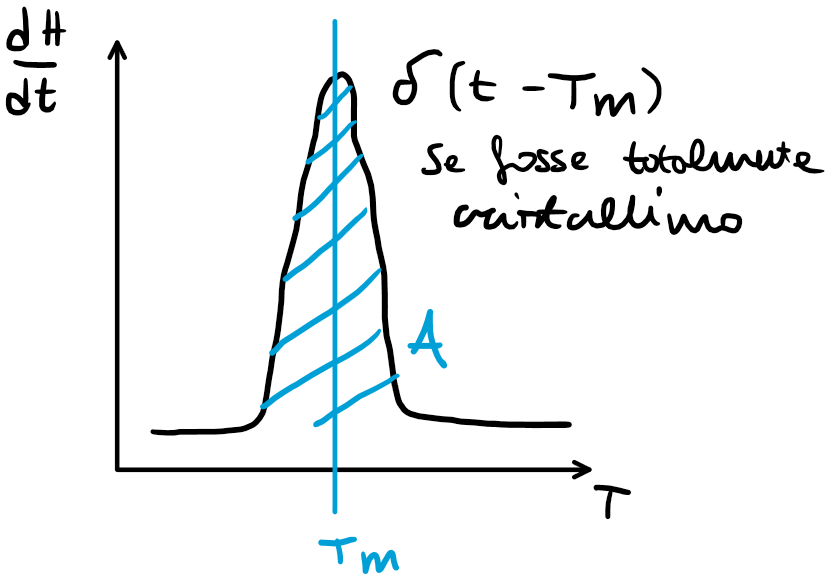
\includegraphics[width = \textwidth]{gfx/DSC}
\caption{Esempio di misura DSC}
\label{fig:DSC}
\end{figure}

L'area di calore latente è in genere più grande dell'area di cristallizzazione forzata se si vuole sapere quanto fosse la cristallizzazione prima di questo processo, col materiale vetroso, basta fare la differenza tra le due aree.
Questo permette di ottenere delle informazioni su come il materiale è stato prodotto: se il materiale presenta una cristallizzazione residua dopo il processo allora il raffreddamento non è stato eseguito correttamente e non ha cristallizzato a dovere.
LA procedura consiste in due riscaldamenti:
\begin{enumerate}
\item Nel primo riscaldamento si valuta la storia termica del materiale . Quindi si ha una misura di tipo tecnologico . Se si vede una cristallizzazione che si presenta durante la prova , ciò indica che il ciclo tecnologico non è stato effettuato correttamente . Poi si raffredda il materiale con la stessa velocità con cui lo si è scaldato per azzerare la sua storia termica.
\item Nel secondo riscaldamento, si valutano le caratteristiche del materiale perché dopo il primo riscaldamento si è azzerata la storia termica: per cui si possono valutare le caratteristiche del materiale come se fosse "vergine". Se non si presenta più cristallizzazione allora vuol dire che il materiale ha subito una cristallizzazione forzata. Altrimenti è un materiale che cristallizza per motivi cinetici più che termodinamici.
\end{enumerate}
Confrontando le tue caratteristiche si ottengono le informazioni definitive sul materiale.

\begin{equation}
\frac{dH}{dt} \rightarrow \frac{\frac{dH}{dt}}{\dot{T}} = \frac{\frac{dH}{dt}}{\frac{dT}{dt}} = \frac{dH}{dt}
\end{equation}
Da cui:
\begin{equation}
C_p = \frac{dH}{dT} \rightarrow c_p = \frac{1}{M}\frac{dH}{dT}
\end{equation}
Quello che si vede dalla calorimetria non è altro che la variazione dl calore specifico in funzione della temperatura.

Si osserva che il calore specifico quando attraversa la transizione vetrosa, aumenta con discontinuità. Resta più o meno invariato (aumenta leggermente) meò caso della fluidificazione del materiale.

Alcuni strumenti mostrano le termografie in funzione del calore assorbito o rilasciato. In genere si riconoscono perché hanno una dicitura \textbf{EXO} o \textbf{ENDO} per indicare cosa viene considerato come convenzione positiva.
Di fatto, la termografia ha comunque lo stesso comportamento.
Alle volte viene normalizzata la potenza termica sul peso, mostrando così il calore specifico.

Se si presentano più picchi endotermici, possono rappresentare:
\begin{itemize}
\item Due materiali miscibili l'uno dentro l'altro. Quindi prima fonde un polimero poi il secondo. Di solito succede quando viene addizionato il colorante, in forma di polveri di tipo ceramico che viene \textit{portata dentro} tramite l'aggiunta di un ulteriore polimero detto \textbf{polimero trasportatore}. Di solito si tratta di una resina al alta densità.
\item Se si ha un copolimero a blocchi, a patto che i due blocchi siano sufficientemente grandi.
\end{itemize}

Durante il raffreddamento possono presentarsi più picchi esotermici di cristallizzazione.

Da cui si può vedere che la \ac{DSC} è una misura estremamente versatile.

Se si presentano dei picchi, verso il basso, dopo la il fenomeno della fusione dei cristalli, questi indicano dei processi di degradazione del materiale.

Ad esempio il Teflon ha una temperatura di degradazione più bassa di quella di fusione. Infatti il Teflon non può essere processato per fusione.